\subsection{Open Source, GPU-accelerated, Finite-Difference, Time-Domain
    Software for Shear Wave Elastography Simulation (Dr.\ McAleavey)}

\subsubsection{Summary}
Two finite difference time domain codes have been created for the purpose of
simulating shear wave propagation: a 2D ``C-plane'' simulator allowing for
arbitrary viscoelastic models in a plane normal to the push beam, and a 3D
``B-scan'' simulator using a Kelvin-Voigt viscoelastic model. The 3D simulator
includes a tool for simulation of realistic push beams by full wave simulation
of acoustic propagation from a definable aperture, and allows modeling of sound
speed variations in the target, as well as variations in shear wave speed. A
description of the simulators and representative output is presented, along
with a comparison of simulated and measured output in the QIBA Phase II set 1
phantoms. Differences in the measured and simulated output are observed, and
will be examined in future work. 

\subsubsection{Description of the Simulators}

\paragraph{C-plane simulator}
The C-plane simulator is based on a Kelvin-Voigt model based simulation similar
to that described in~\cite{Orescanin2011} was implemented. This 2D simulation
utilizes split field equations and perfectly matched layers (PMLs) implemented
on a Yee cell grid as originally proposed in~\cite{Berenger1994}. This
simulator is capable of modeling non-axisymmetric beams, as for instance those
produced at the focus of a rectangular aperture. The simulator is limited to
modeling a single plane normal to the push beam axis, and assumes that the
material and push beam do not vary along the beam axis. 

For the simulations shown here the modeled domain is 10 cm x 10 cm in the
elevational-lateral plane with 1 cm PML on all domain edges. The simulation
step size is 0.4 mm spatially and 1 $\mu$s temporally. Finally, this
implementation includes an iterative guess and revise scheme for calculating
time derivatives.  This involves first calculating the time update using a
linear model and then iteratively solving for the viscoelastic update. 

To produce the simulated shear wave data, an initial axial velocity is applied
to the simulation domain that approximates the focal geometry of the STL-SWEI
pushing pulse. Specifically, a Gaussian cylindrical excitation with a lateral
full width at half max (FWHM) of 1 mm was applied to the center of the
simulation grid for 300 $\mu$s. This excitation time was used to approximate the
upper limit of ARFI excitation time used in our experiments. The data from the
simulation was sampled at a rate of 7.44 kHz. Subsequently, this data is
interpolated and stored in a data structure is identical to that used for
actual RF processing in our in-house software. Therefore, the simulation data
can be used to directly test the actual code used for processing ultrasound
images. 

Representative simulator outputs are shown in Figure~\ref{fig:steve-representative-output}.

\begin{figure}[htb!]
    \centering
    \begin{tabular}{cc}
        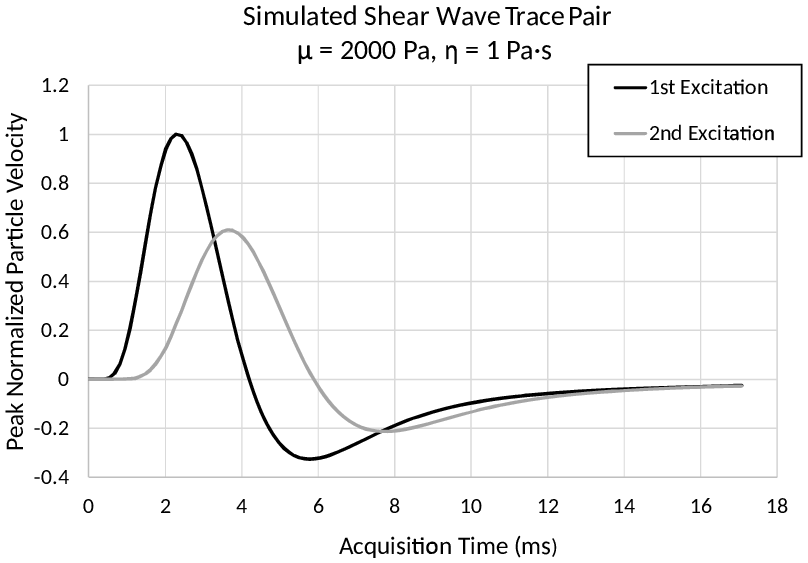
\includegraphics[width=0.45\linewidth]{steve/figs/image1.png} &
        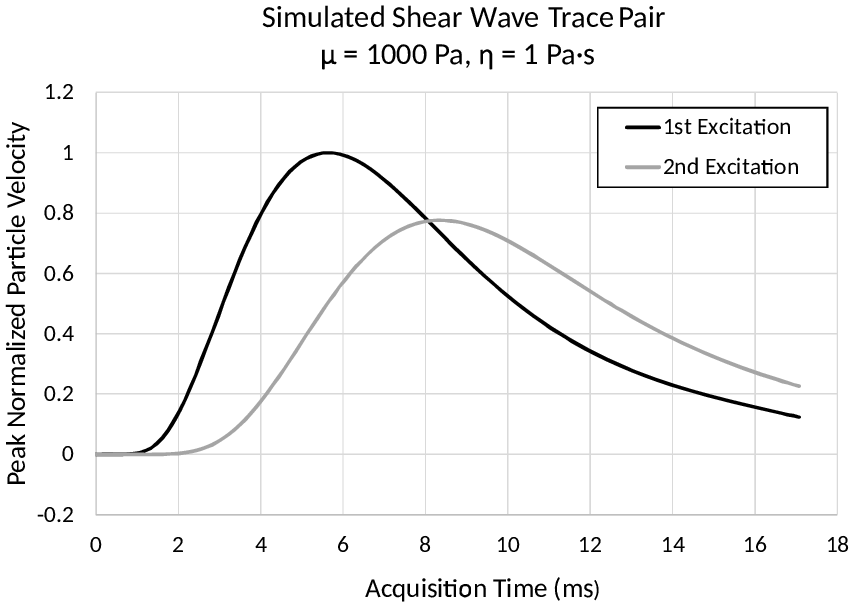
\includegraphics[width=0.45\linewidth]{steve/figs/image2.png} \\
    \end{tabular}
    \caption{Representative simulator output data} 
\label{fig:steve-representative-output}
\end{figure}

\paragraph{B-mode simulator--``Elasticity Lab Simulator''}
The ``B-plane'' simulator permits simulation of both the ultrasonic ``push
beam'', as well as the resulting shear wave. The simulation flowchart is
depicted in Figure~\ref{fig:steve-sim-flowchart}. Either the result of an
acoustic wave simulation, or an arbitrarily specified forcing function, is
applied as input to the full-wave KV simulator to determine motion in response
to an excitation. 

\begin{figure}[htb!]
    \centering
    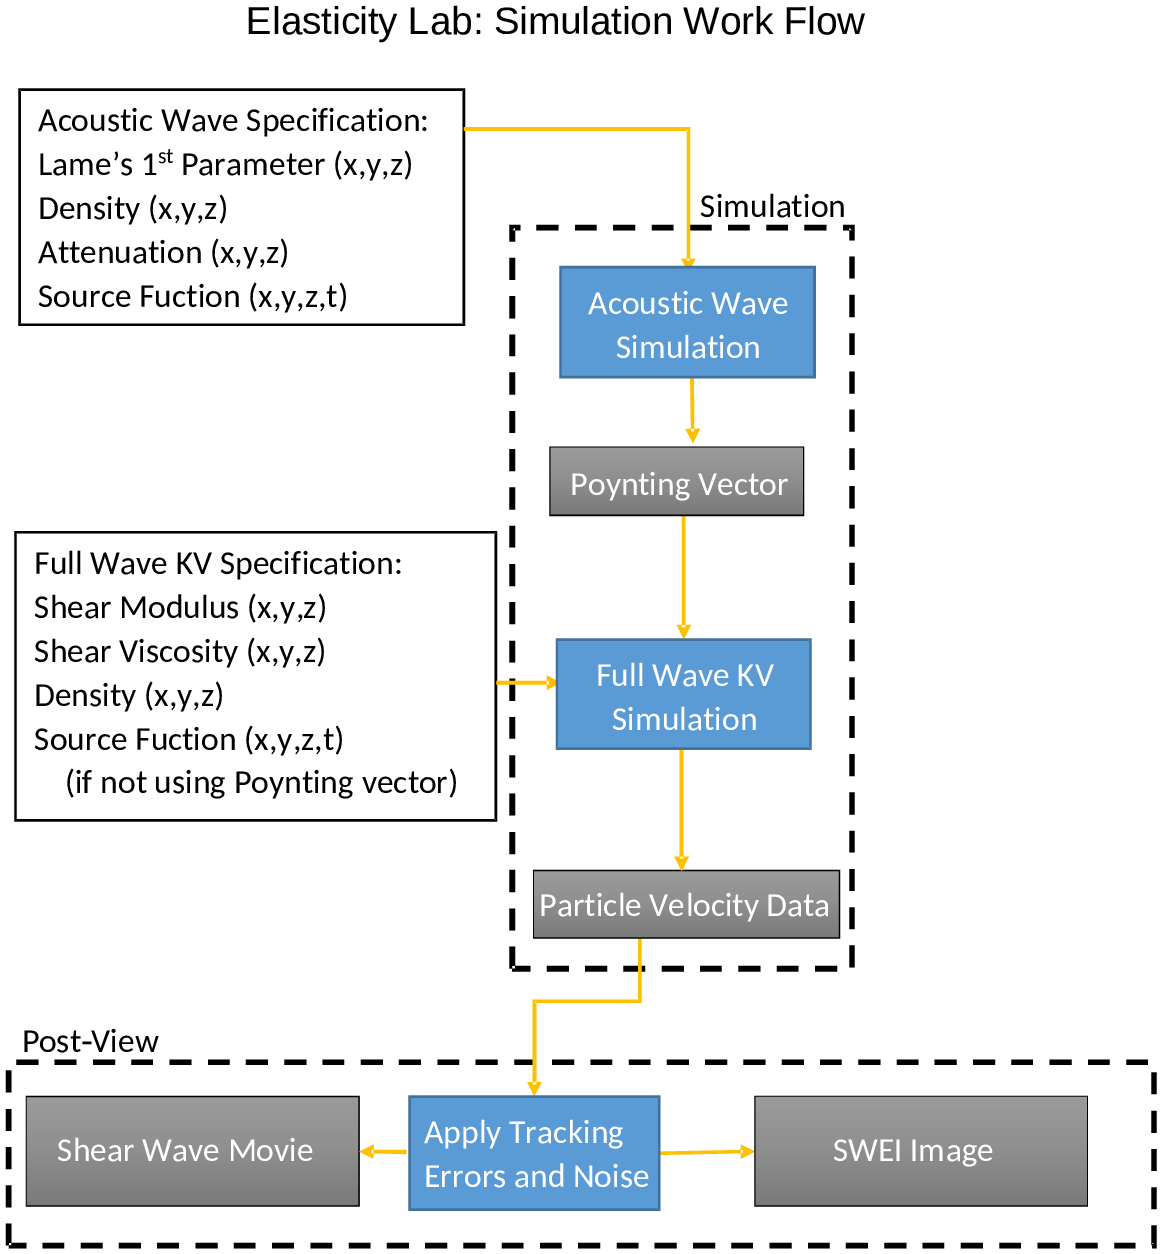
\includegraphics[width=0.75\linewidth]{steve/figs/image3.png}
    \caption{Flowchart depicting the stages and code involved in the overall
    shear wave elastography simulation.} 
\label{fig:steve-sim-flowchart}
\end{figure}

The acoustic wave simulator allows calculation of push beam geometry and
forces. Beginning with acoustic parameters of the medium (Lame’s first
($\lambda$) parameter, attenuation, and density as functions of position) and
the acoustic source (aperture) as a function of position and time, an acoustic
wave simulation is run to determine the Poynting vector associated with the
push beam, from which both the magnitude and direction of the acoustic
radiation force are calculated.  This forcing function may then be applied to
the full wave KV simulator. 

The forcing function from the acoustic wave simulator, or an arbitrary
user-specified forcing function, along with material parameters (modulus,
viscosity, and density as functions of position) are the inputs to the full
wave KV simulator (Figure~\ref{fig:steve-UI}). This simulator models the
mechanical response of the described target, providing particle velocity as a
function of position and time. Performing the entire simulation with realistic
longitudinal wave speeds would take a prohibitive amount of time. Therefore, in
the full wave simulation, the longitudinal wave speed is substantially
decreased (10 - 100 m/s) to allow larger time steps to be used and increasing
the speed of the simulation. 

\begin{figure}[htb!]
    \centering
    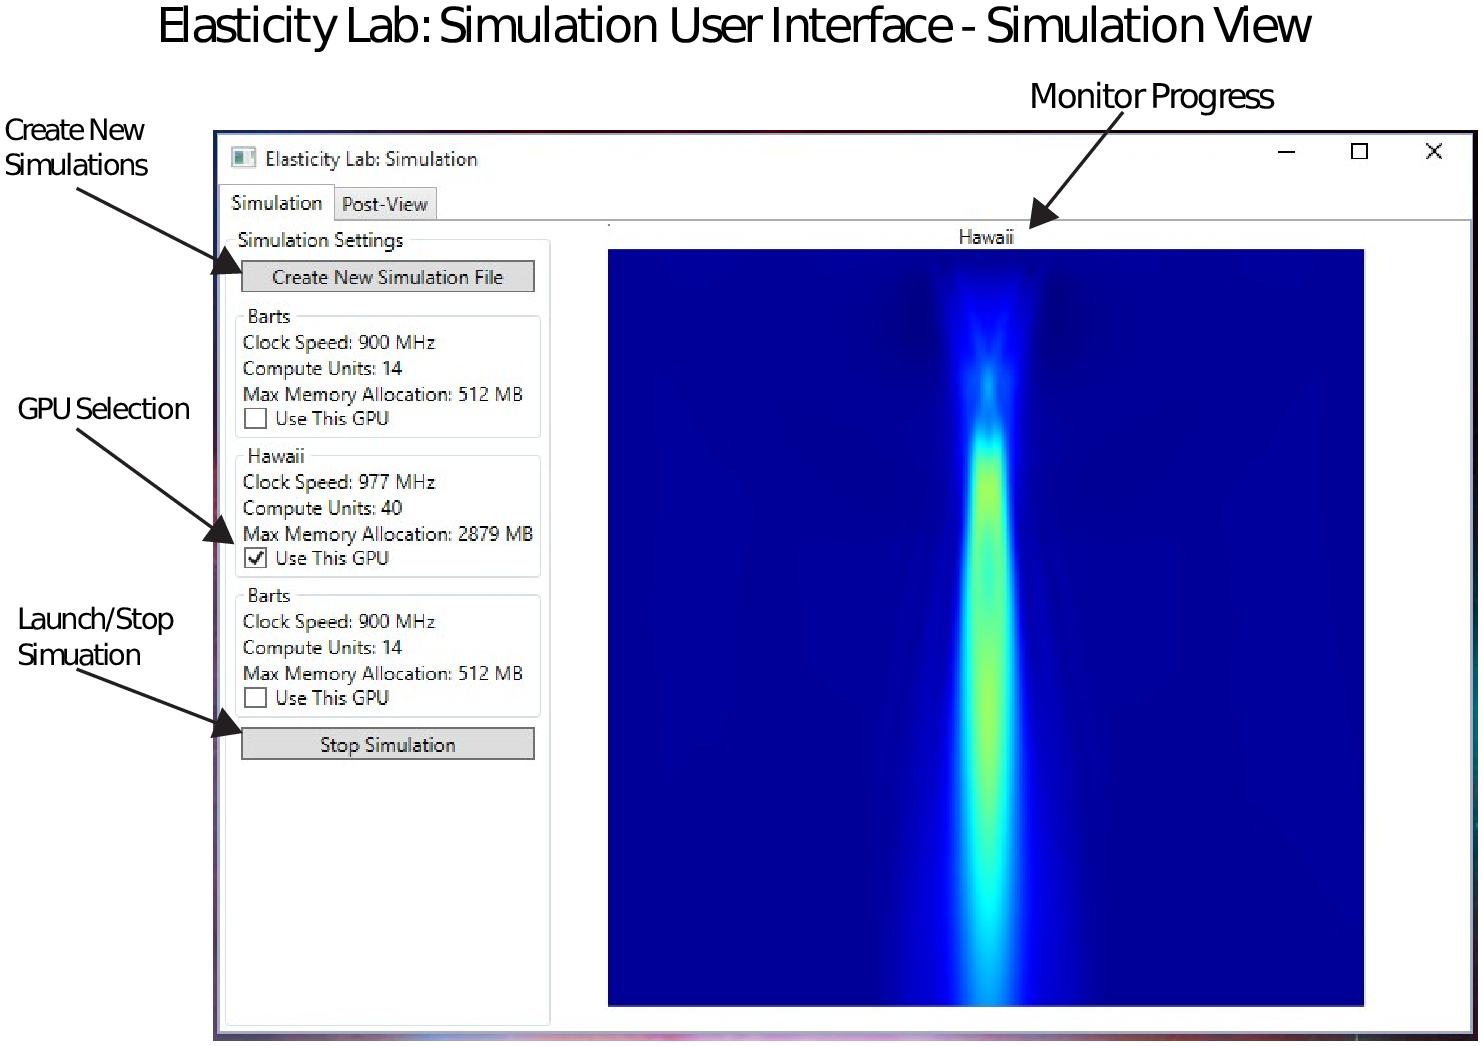
\includegraphics[width=0.75\linewidth]{steve/figs/image4.png}
    \caption{User interface for the acoustic wave simulator, used to model the
    acoustic radiation force push beam.} 
\label{fig:steve-UI}
\end{figure}

The files generated by the simulator can be opened in a post-view code allowing
visualization of the motion. The user interface for this part of the simulation
is depicted in Figure~\ref{fig:steve-post-UI}. In this part of the software, speckle
bias can be approximated and noise added to the data. Shear wave propagation
videos may be produced inside the interface. The data may then be processed
into SWEI images with user defined tracking offsets and push beam spacing
(beam ensemble settings). Because this SWEI specific functionality is in the
last step of the simulation work flow, images using various beam ensemble
settings may be produced. The files may also be opened in Matlab.

\begin{figure}[htb!]
    \centering
    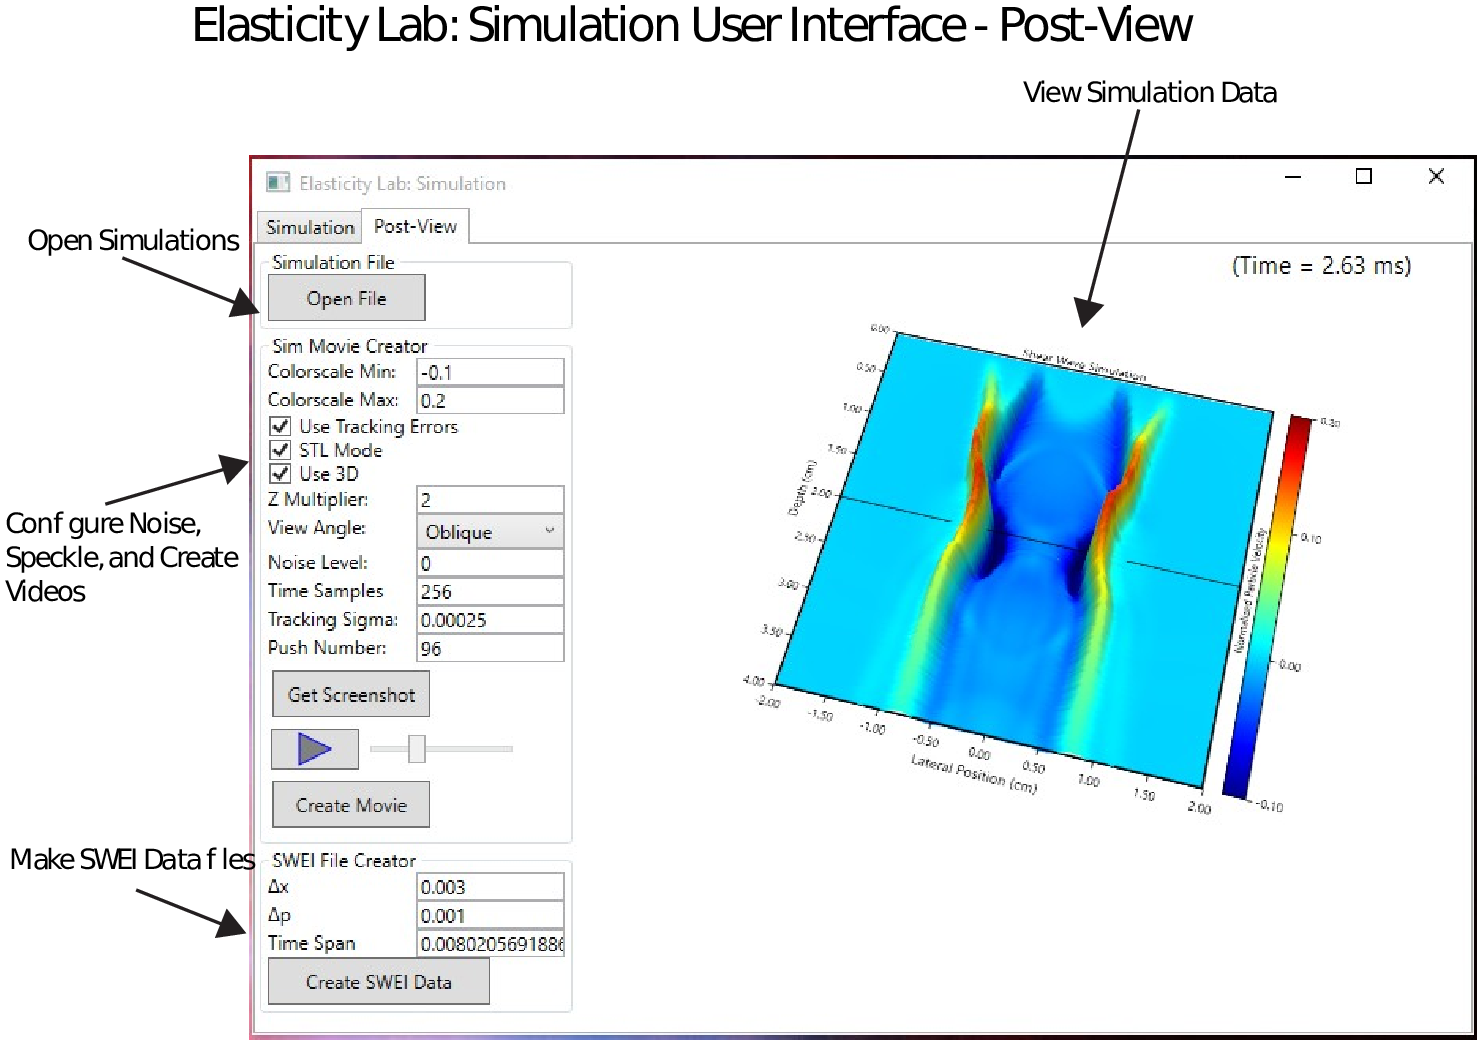
\includegraphics[width=0.75\linewidth]{steve/figs/image5.png}
    \caption{User interface for the acoustic wave simulator, used to model the
    acoustic radiation force push beam.} 
\label{fig:steve-post-UI}
\end{figure}

\paragraph{Acoustic Wave Simulation}
The acoustic wave simulation is based on the acoustic wave equations in the
velocity stress formulation. In this formulation, the particle velocity and the
stress (or pressure) are related by a pair of first order differential
equations. They may be expressed as:
\begin{align*}
\rho \frac{\delta v}{\delta t} = \nabla P\\
\frac{\delta P}{\delta t} = \Lambda \nabla \cdot v,
\end{align*}
where $v$ is the velocity, $P$ is the pressure, $\rho$ is the density and
$\Lambda$ is Lame's first parameter.  We use the capital $\Lambda$ here to
distinguish it from the wavelength, $\lambda$. Although the equations could be
combined to arrive at a second-order differential equation, the first order
equation are more convenient for discretization using finite difference method.
Using the so-called staggered grid depicted (Figure~\ref{fig:steve-staggered-grid}), the differential
equations may be split into component parts and discretized as:

\begin{gather*}
    v_x^{i+\frac{1}{2},j,k,n+1} = v_x^{i+\frac{1}{2},j,k,n} + 
                                  \frac{1}{\rho}\frac{P^{i+1,j,k,n+\frac{1}{2}}-P^{i,j,k,n+\frac{1}{2}}}{\Delta x}\\
    v_y^{i,j+\frac{1}{2},k,n+1} = v_y^{i,j+\frac{1}{2},k,n} + 
                                  \frac{1}{\rho}\frac{P^{i+1,j,k,n+\frac{1}{2}}-P^{i,j,k,n+\frac{1}{2}}}{\Delta y}\\
    v_z^{i,j,k+\frac{1}{2},n+1} = v_z^{i,j,k+\frac{1}{2},n} + 
                                  \frac{1}{\rho}\frac{P^{i+1,j,k,n+\frac{1}{2}}-P^{i,j,k,n+\frac{1}{2}}}{\Delta z}\\
    P^{i,j,k,n+\frac{1}{2}} = P^{i,j,k,n-\frac{1}{2}} + \Lambda \Delta t 
                              \left( 
                                    \frac{v_x^{i+\frac{1}{2},j,k,n}  - v_x^{i-\frac{1}{2},j,k,n}}{\Delta x} +
                                    \frac{v_y^{i,j+\frac{1}{2},k,n}  - v_y^{i,j-\frac{1}{2},k,n}}{\Delta y} +
                                    \frac{v_z^{i,j,k+\frac{1}{2},n}  - v_z^{i,j,k-\frac{1}{2},n}}{\Delta z}
                              \right)
\end{gather*}

Here $i$, $j$, and $k$ are discrete integer coordinates in the $x$, $y$, and
$z$ dimensions, respectively. The discretization of the time dimension is given
by the integer $n$. Consequently, the discrete time-space coordinates ($i, j,
k, n$) map to the real valued coordinates ($i \Delta x$, $j \Delta y$, $k\Delta
z$, $n \Delta t$). Each dimension is staggered into half steps, with the
velocity calculated at integer multiples of time and the pressure calculated at
half-integer multiples. 

\begin{figure}[htb!]
    \centering
    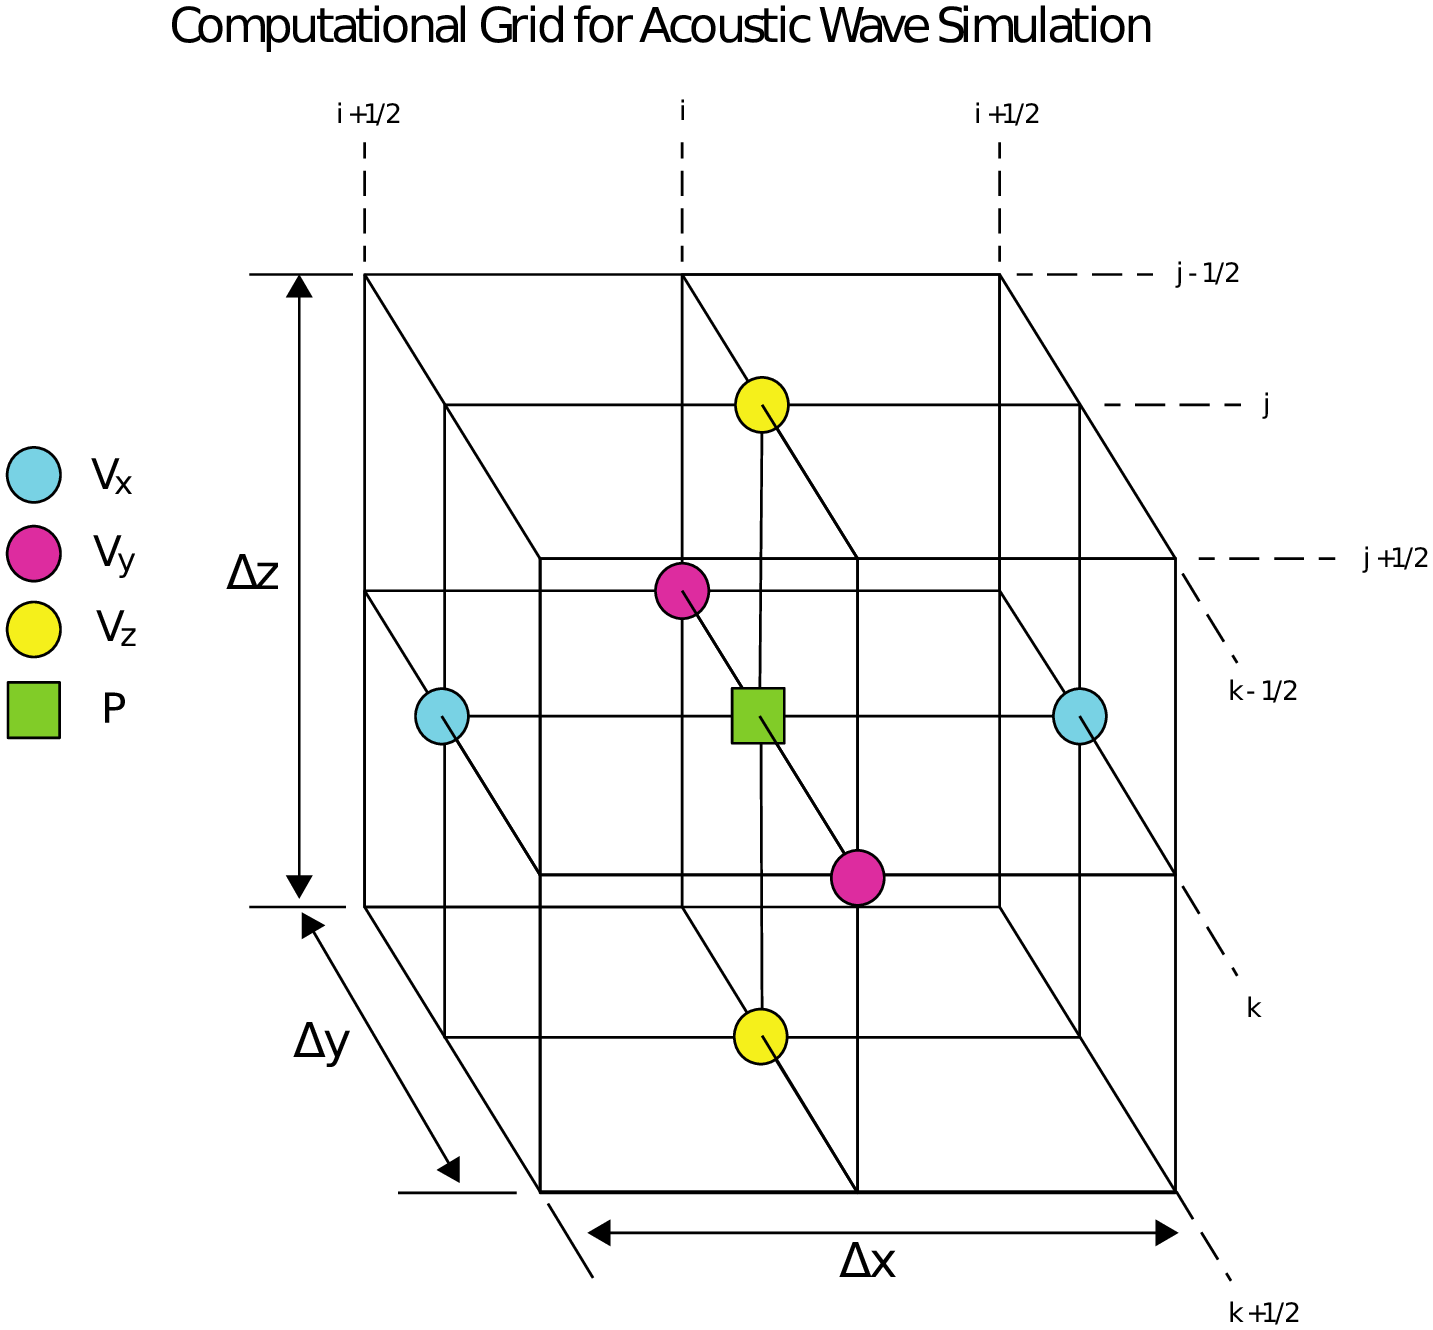
\includegraphics[width=0.75\linewidth]{steve/figs/image6.png}
    \caption{Computational grid for acoustic wave simulation.} 
\label{fig:steve-staggered-grid}
\end{figure}

Grid dispersion is minimized by choosing a grid step size that is less than
one-tenth of the shortest shear wave wavelength. Once the step size is chosen
the time step is set using the Courant-Friedrichs-Lewy (CFL) condition. This is
given as:
\begin{equation*}
    \Delta t \leq \frac{\sqrt{3}}{c \sqrt{\left( \frac{1}{\Delta x}\right)^2 +
    \left( \frac{1}{\Delta y}\right)^2 + \left( \frac{1}{\Delta z}\right)^2}}.
\end{equation*}
Since this FDTD solver is used primarily for simulated mono-frequency
excitation, attenuation may be accounted for by simply introducing a frequency
independent attenuation. This would not be adequate for simulating pulse-echo
imaging where there is pulse has a broad spectrum. However, for the purpose of
simulating an ARF beam, the long duration of the pulse diminishes the effect of
any transients yielding a narrow spectrum. To achieve what amounts to an
exponential decay law, the velocity update equation are rewritten as:

\centerline{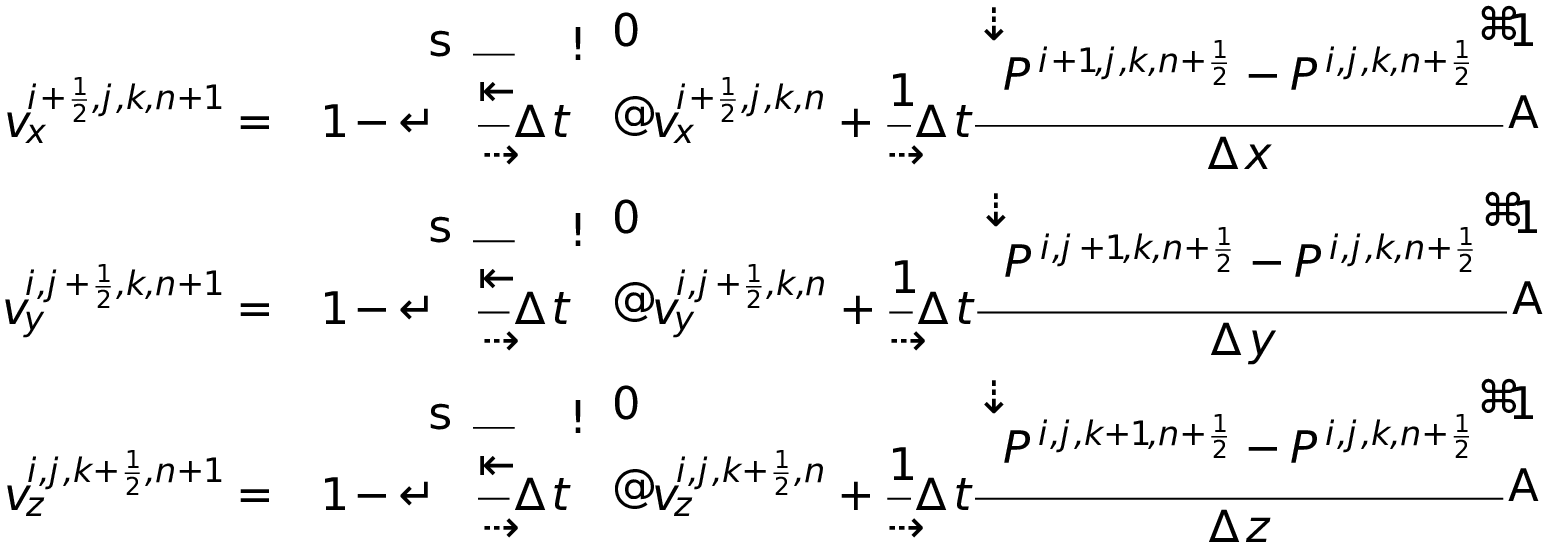
\includegraphics[width=0.65\linewidth]{steve/figs/image8.png}}

At the boundaries of the computational domain, the velocity outside the grid is
taken to equal that immediately inside. Let $I$, $J$, and $K$ be the lengths of
the computational grid in the $i$, $j$, and $k$ directions, respectively. The
boundary conditions may be written as: 

\centerline{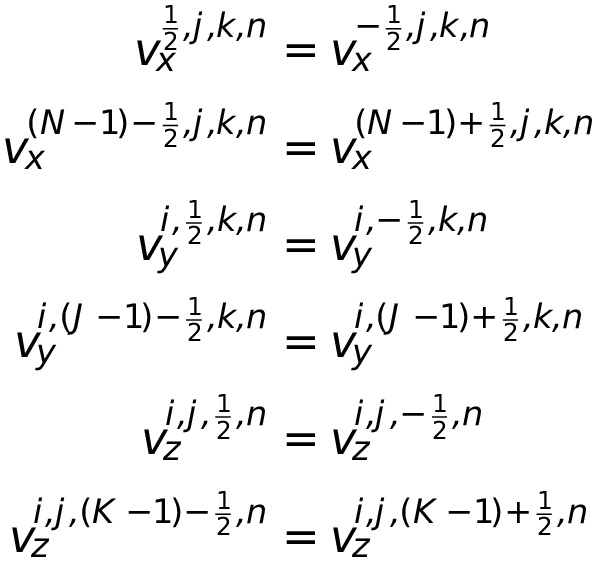
\includegraphics[width=0.3\linewidth]{steve/figs/image9.png}}

Note that these conditions are the same as stating that the derivative of the
velocity across the boundary is zero. We simply skip calculating the derivative
across the boundary to implement this. However, these are reflective boundary
conditions. In order to prevent reflections, the outer several cells of the
computational domain are replaced by perfectly matched layers (PMLs). The PML
is implemented by splitting the update equations for the perimeter of the grid
into separate equations for each individual spatial derivative and the
weighting each derivative by a scaling factor. This is referred to as operator
stretching. For the velocity case, there is only one spatial derivative to
begin with and so the 
number of equations is unchanged. The velocity PMLs are given by:

\begin{gather*}
    v_x^{i+\frac{1}{2},j,k,n+1} = C_x v_x^{i+\frac{1}{2},j,k,n} + 
                                  D_x \frac{1}{\rho}\frac{P^{i+1,j,k,n+\frac{1}{2}}-P^{i,j,k,n+\frac{1}{2}}}{\Delta x}\\
    v_y^{i,j+\frac{1}{2},k,n+1} = C_y v_y^{i,j+\frac{1}{2},k,n} + 
                                  D_y \frac{1}{\rho}\frac{P^{i+1,j,k,n+\frac{1}{2}}-P^{i,j,k,n+\frac{1}{2}}}{\Delta y}\\
    v_z^{i,j,k+\frac{1}{2},n+1} = C_z v_z^{i,j,k+\frac{1}{2},n} + 
                                  D_z \frac{1}{\rho}\frac{P^{i+1,j,k,n+\frac{1}{2}}-P^{i,j,k,n+\frac{1}{2}}}{\Delta z}\\
\end{gather*}

Here $Cx, Cy, Cz$ and $Dx, Dy, Dz$ are the PML scaling factors for the $x, y,$
and $z$ derivatives, respectively. Notice that $Dx, Dy,$ and $Dz$ replace the
time step in the equations. These coefficients for the x dimension are given
by:
\begin{align*}
    C_x = e^{-s_x \Delta t}\\
    D_x = \frac{1-C_z}{s_x},
\end{align*}
and the equations for the other dimensions are the same with substitution of
the subscript. The term $s_x$ is an attenuation that is set as desired to
achieve good absorption of the incident wave. Typically this value is increased up
exponentially from zero at the inner edge of the PML to some maximum value at
the domain’s outer edge.

Implementing of the FDTD model on the GPU requires consideration of memory
access.  In our implementation, the data is laid out with the depth, $z$,
dimension leading. On AMD GPUs, GPU threads come in batches of 256 called
work-groups.  Since GPU performance relies critically on adjacent threads
accessing adjacent data, in our implementation each work group is assigned 256
adjacent point on the FDTD grid vertically. However, this requires that the
depth dimension be a multiple of 256. Therefore, once the step size is
determined the depth of the grid must be 256 ∗ $\Delta$z ∗ m for some integer
m. When the grid is not a multiple of 256 then the work-group size is reduced
to some power of 2 that will fit the grid. For odd numbered grid lengths only
one thread per work-group may be assigned. Thus, choosing the correct grid size
can result in an up to 256x boost in performance. 

In addition to memory access optimizations, the memory usage in our
implementation is minimized by using functions to represent the material
parameters rather than arrays of values. This reduces the total memory needed
and the number of accesses to the GPUs global memory that is required. These
functions are defined in the specification files. They may then be compiled
into the core FDTD program at run-time. 

\paragraph{Full Wave Kelvin-Voigt Simulation}
The full wave simulation is similar to that describe for the acoustic wave
case; however, the full stress tensor, $T$ , is calculated rather than just the
pressure, $P$. The computational grid used in the implementation is shown in
Figure~\ref{fig:steve-full-wave-grid}. The three diagonal components of the
stress tensor ($Txx, Tyy, Tzz$) now replace the pressure at the center of the
unit cube. For the isotropic media being simulated, the stress tensor is taken
to be symmetric with $T_{xy} = T_{yx}, T_{zx} = T_{xz}$, and $T_{zy} = T_{yz}$.
These off-diagonal components of the stress tensor are computed along the edges
of the unit cube.  The choice of edge assures that the particular stress
component occupies the same plane as the velocity components with the same
subscripts (e.g., $T_{xy}$ share a plane with $vx$ and $vy$). 

\begin{figure}[htb!]
    \centering
    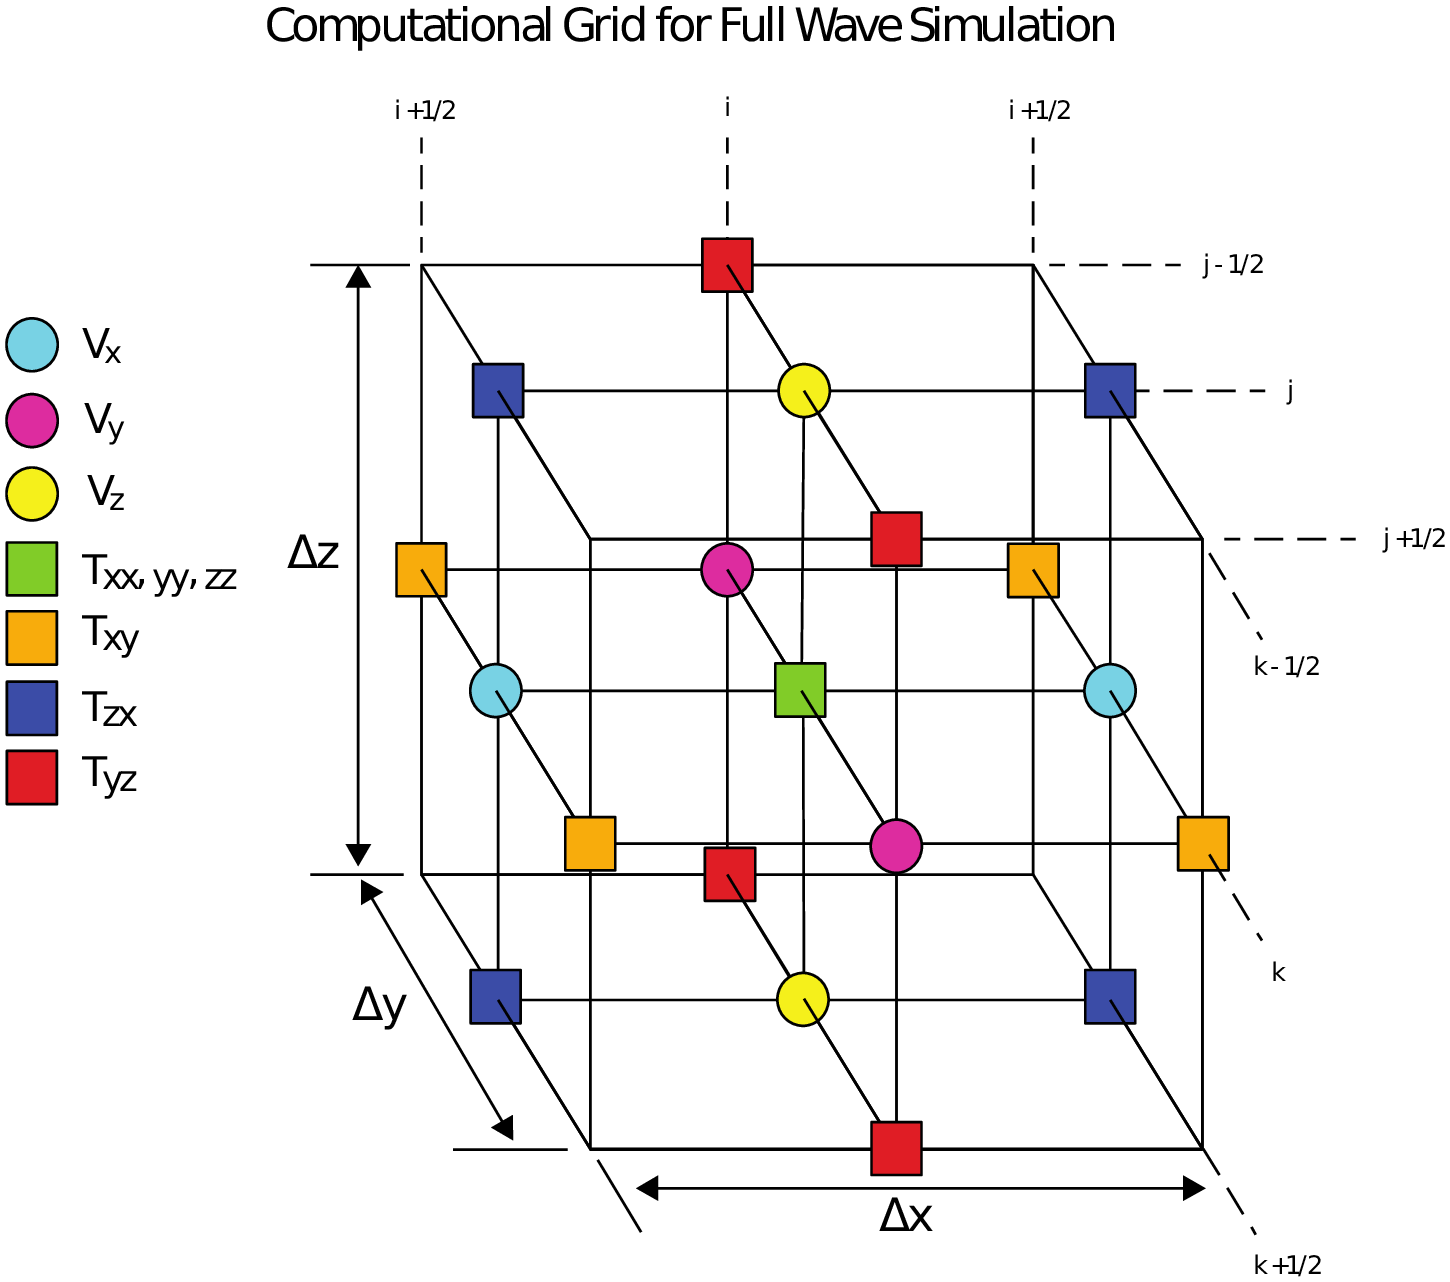
\includegraphics[width=0.75\linewidth]{steve/figs/image11.png}
    \caption{Computational grid for full wave simulation.} 
\label{fig:steve-full-wave-grid}
\end{figure}

\paragraph{Cylindrical Wave Simulations}
The cylindrical wave excitation of a homogeneous media provides a test case for
the accuracy of the 3D simulation. The solution is easily modeled and is built
into our MLE solver. Therefore, the simulation’s accuracy can be readily
verified in this test case. Here a set of five viscoelastic simulations were
performed with cylindrical wave excitations in a 2 kPa shear modulus 3D
simulated material. The shear viscosity was set to either 0.05 Pa$\cdot$s, 0.25
Pa$\cdot$s, 0.50 Pa$\cdot$s, 0.75 Pa$\cdot$s, and 1.00 Pa$\cdot$s. The
simulation viscosity was then validated using the STL-VE algorithm. A 4 cm x 4
cm region of interest was modeled (Figure~\ref{fig:steve-cylindrical-results}). 

\begin{figure}[htb!]
    \centering
    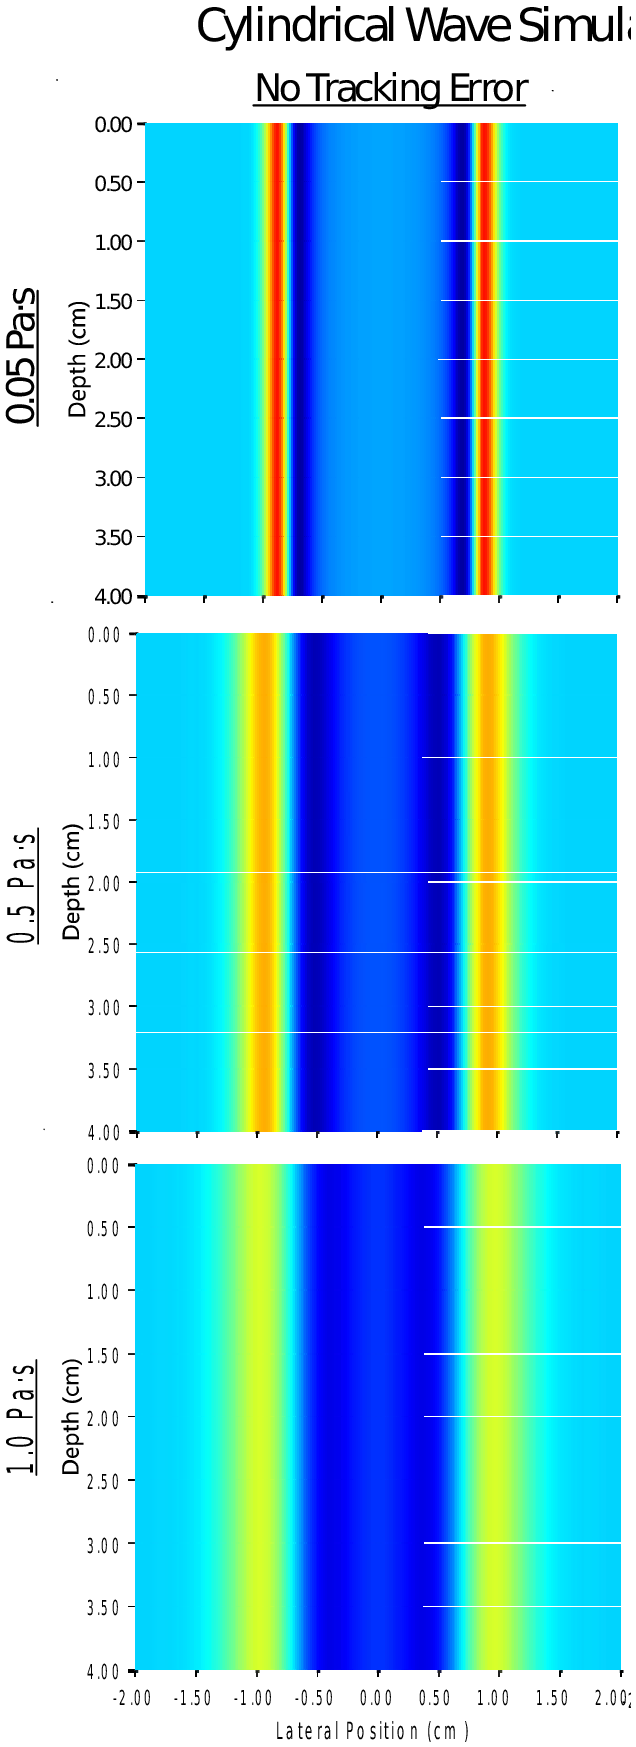
\includegraphics[width=0.3\linewidth, angle=270]{steve/figs/image12.png}
    \caption{Representative frames from simulated cylindrical waves.  A KV
    medium with $\mu$ = 2 kPa an viscosity of 0.05-1 Pa$\cdot$s was modeled for
    verification of the FDTD full wave KV model.} 
\label{fig:steve-cylindrical-results}
\end{figure}

The acoustic wave simulator allows for creation of realistic push beams and
radiation force geometries, allowing examination of potential biases in a
realistic imaging scenario. The panels in
Figure~\ref{fig:steve-full-wave-results} depict simulated typical ARF beam
geometries applied to the Full Wave simulation. The F/\# and the acoustic
attenuation both play a role in determining the shape of the excitation beam.
The simulated beams all utilize a focal depth of 2 cm and a center frequency of
4.21 MHz, matching the phantom experiments. 

\begin{figure}[htb!]
    \centering
    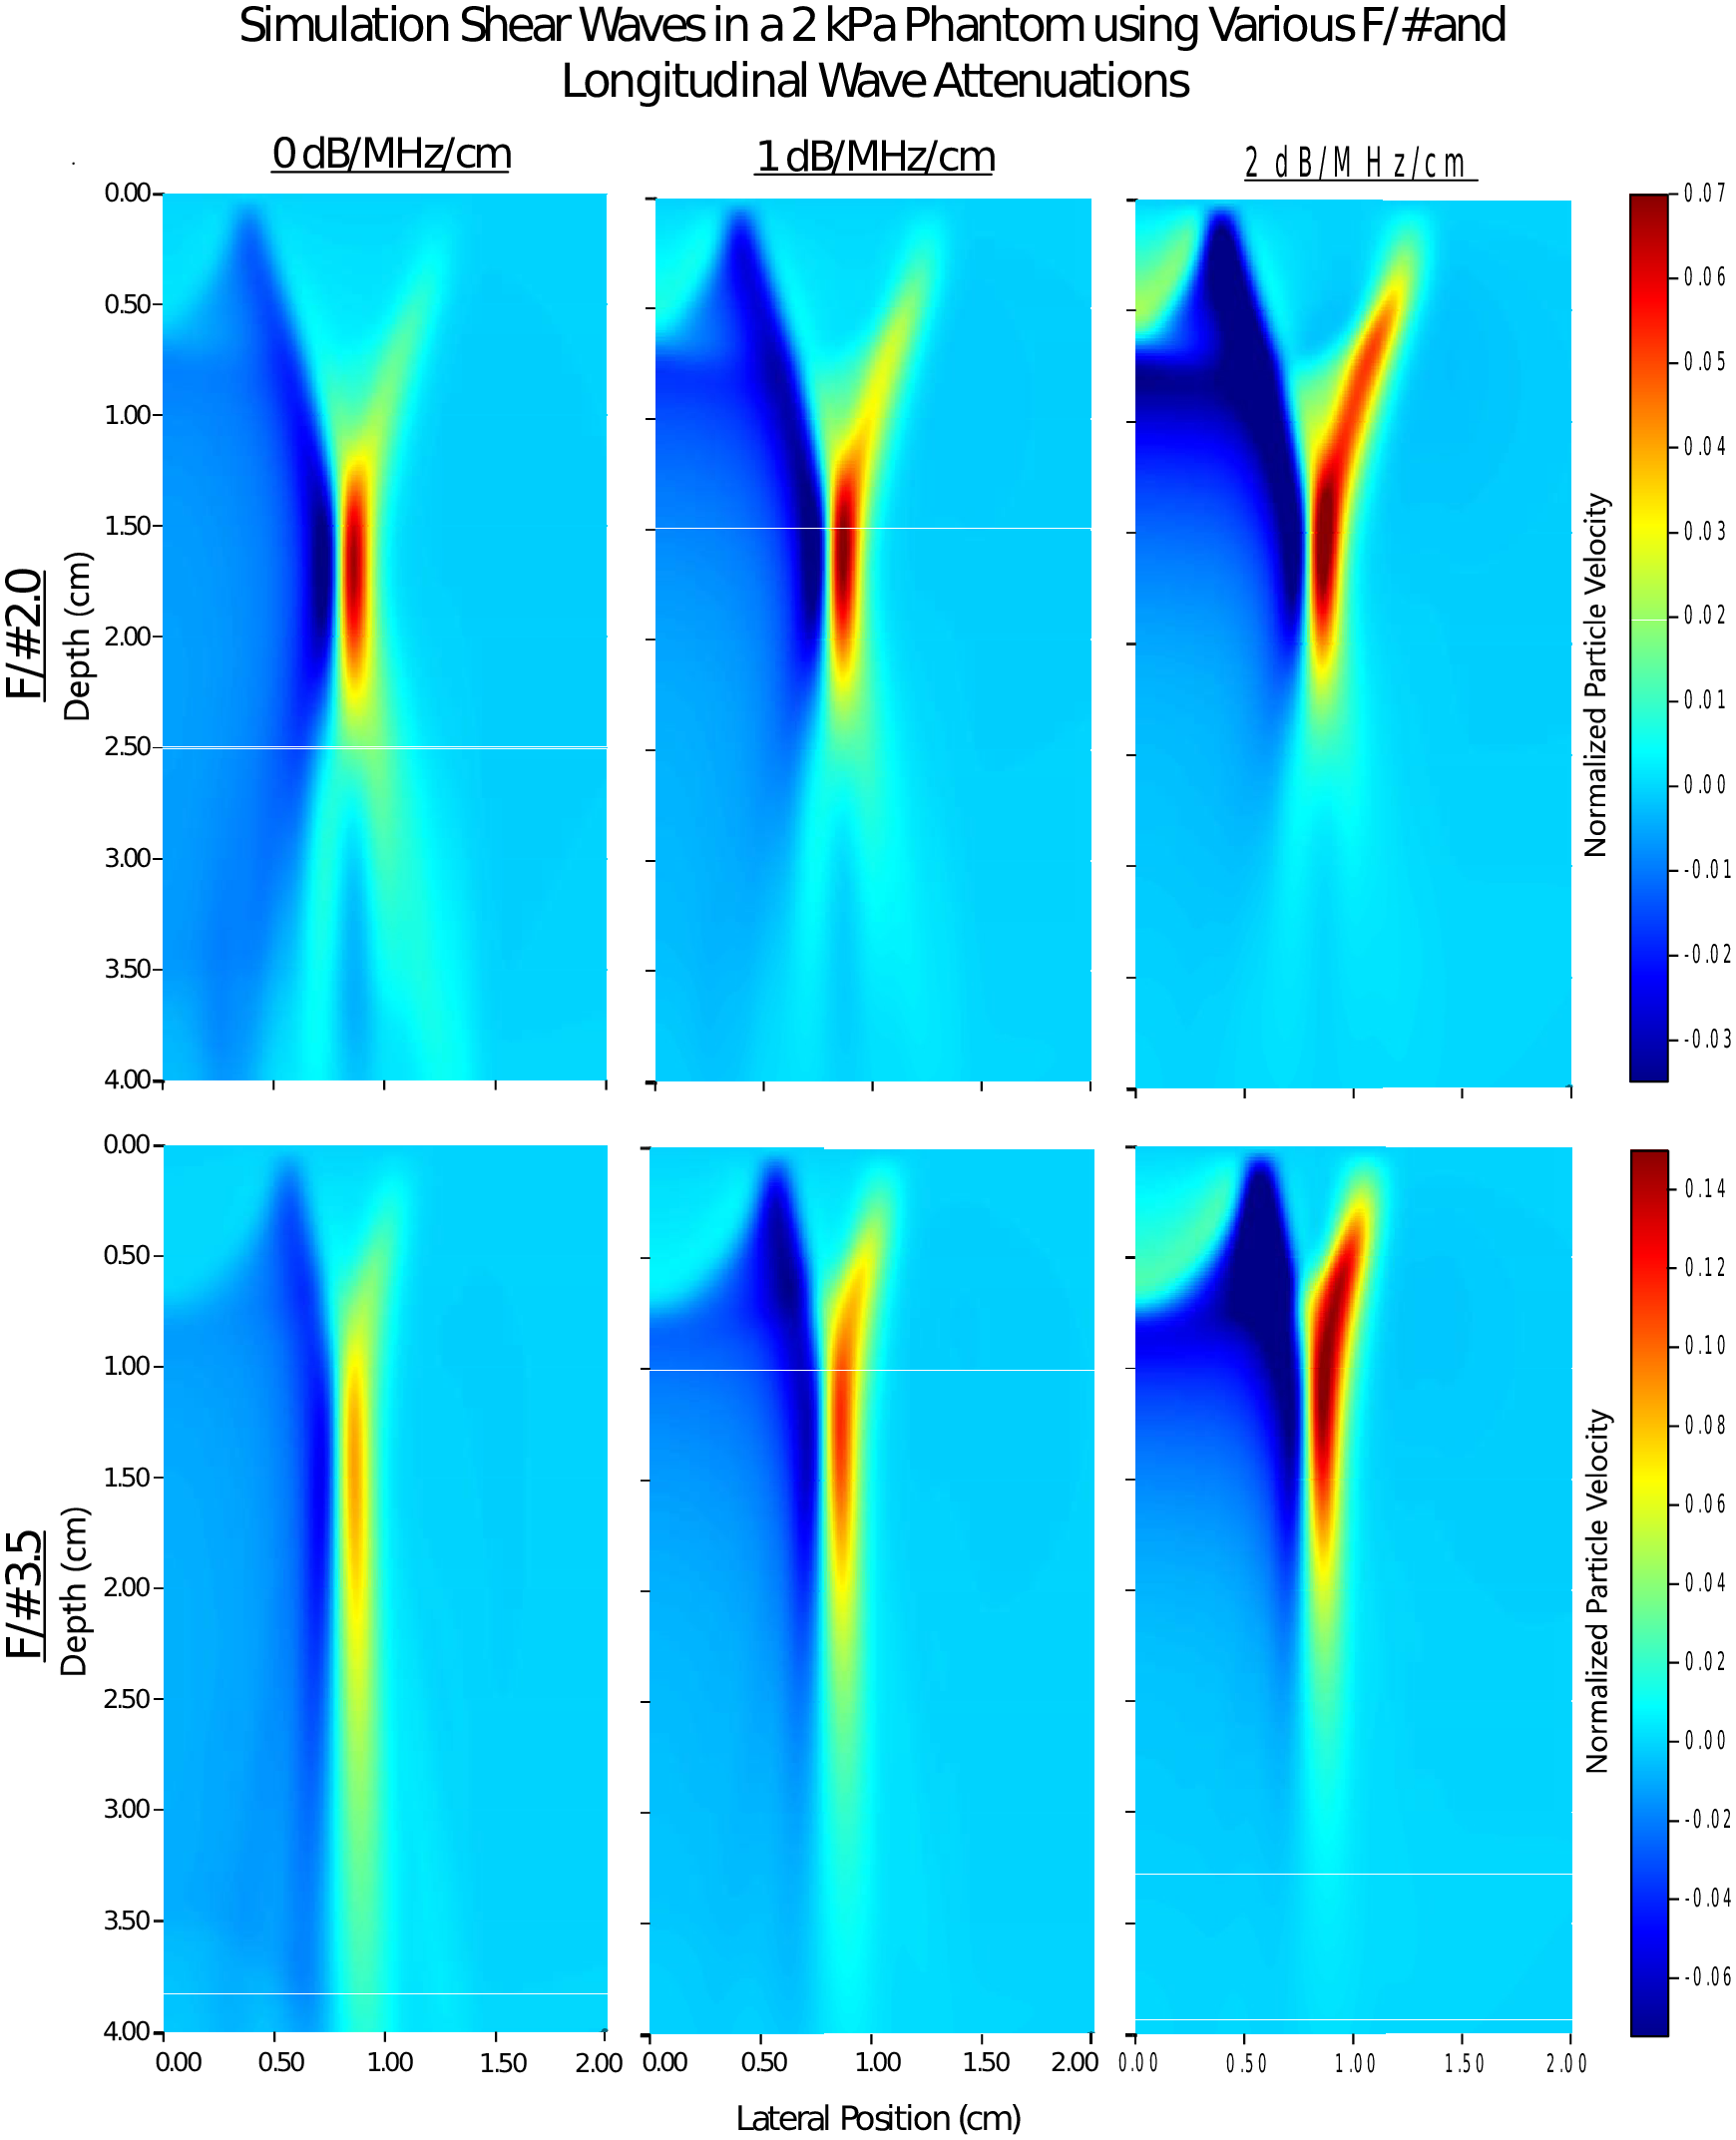
\includegraphics[width=0.75\linewidth]{steve/figs/image13.png}
    \caption{Simulation of shear waves in a 2 kPa phantom using various F/\# and
    longitudinal wave attenuations.}
\label{fig:steve-full-wave-results}
\end{figure}

Distortion of the shear wavefront by inclusions of differing shear modulus from
the background is modeled (Figure~\ref{fig:steve-diffraction}). 

\begin{figure}[htb!]
    \centering
    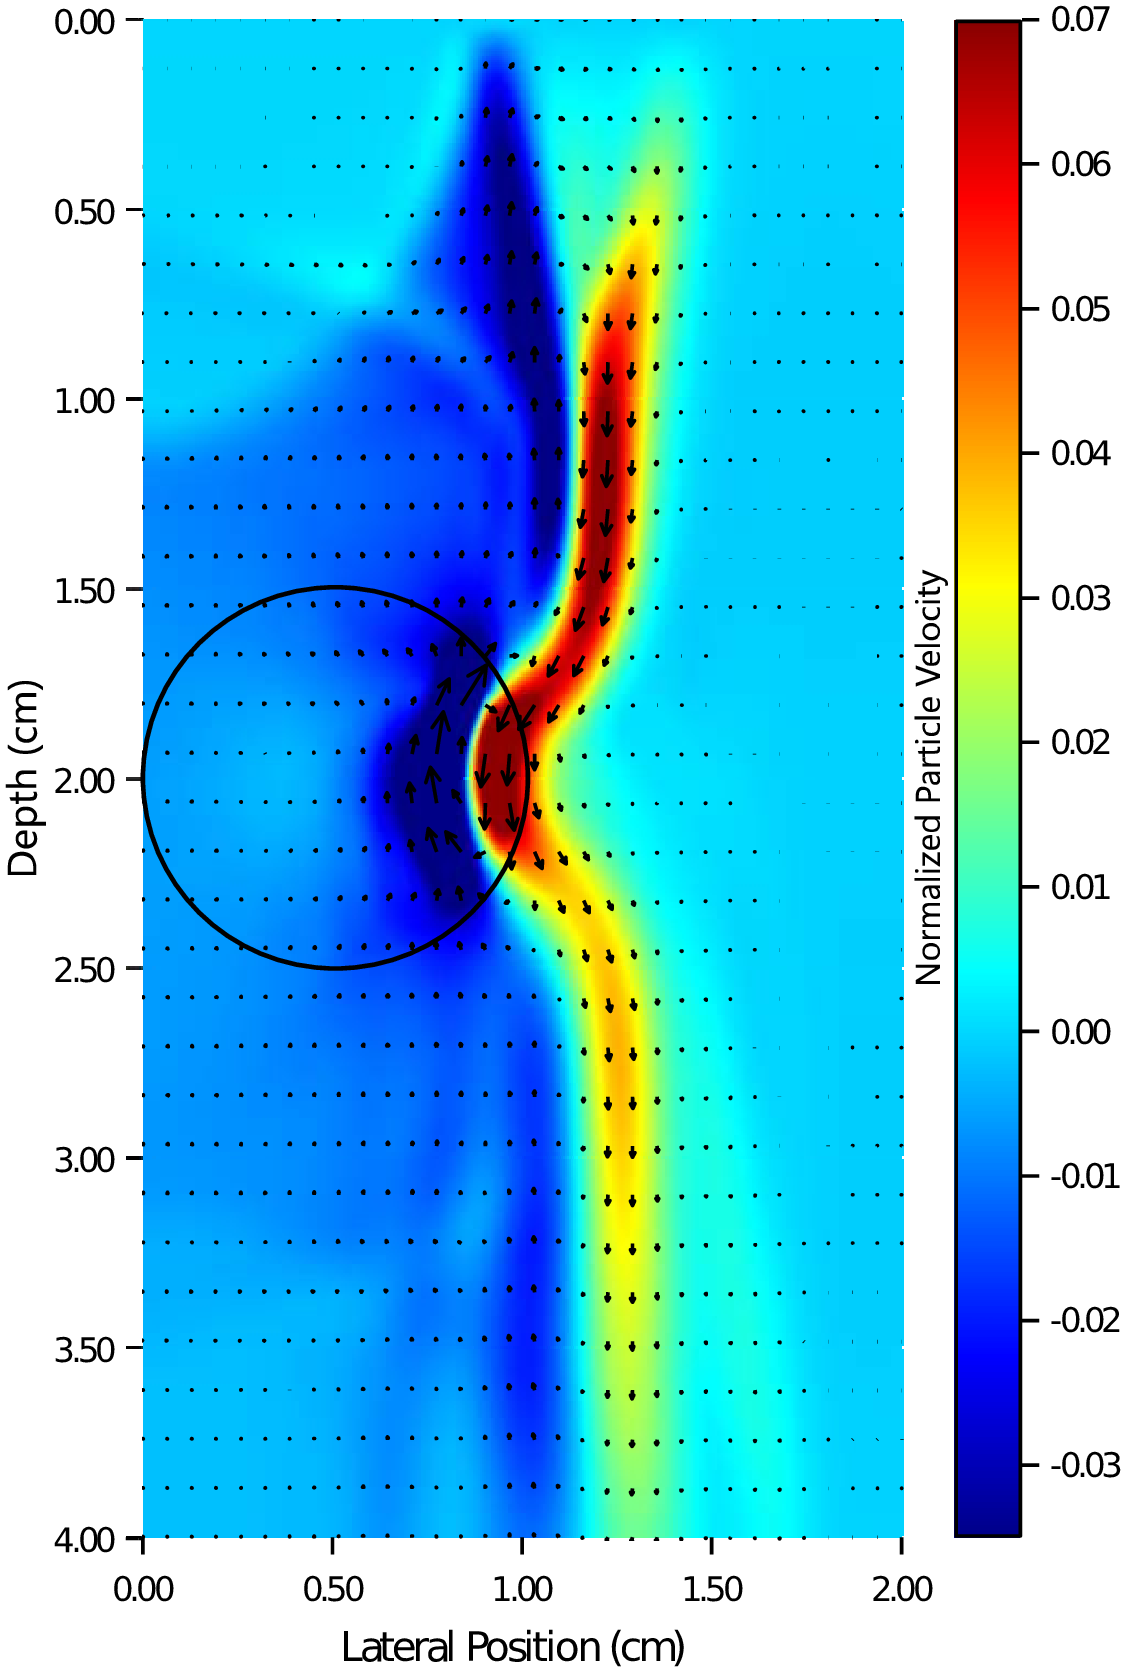
\includegraphics[width=0.4\linewidth]{steve/figs/image14.png}
    \caption{Example of shear wave diffraction by an inclusion.}
\label{fig:steve-diffraction}
\end{figure}

The use of the full wave acoustic simulator allows diffraction of the push beam
to be modeled. Figure~\ref{fig:steve-stl-swei} shows a simulated STL-SWEI image
showing effect of push beam diffraction due to differing acoustic wave speed in
lesion and background, in addition to shear wave speed differences between the
lesion and background. Note that tracking beam diffraction is not simulated.
The boundary of the sphere is depicted by the black circle. Push beam
diffraction effects are observed beneath the lesion. Additionally, the sphere
appears smaller in height than in width with a region of increased modulus
within the bounding circle.

\begin{figure}[htb!]
    \centering
    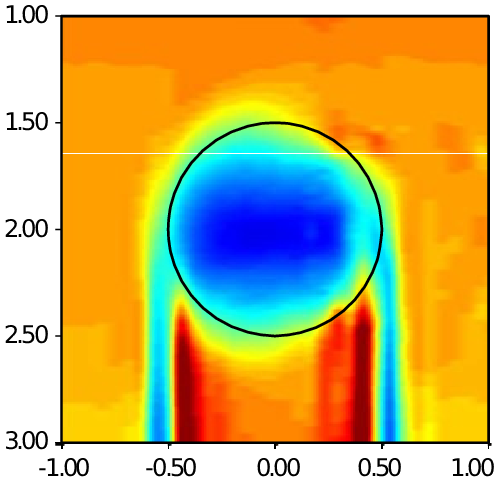
\includegraphics[width=0.3\linewidth]{steve/figs/image15.png}
    \caption{Simulated STL-SWEI image showing the effect of push beam
    diffraction due to differing acoustic wave speed in the lesion and
    background, in addition to shear wave speed differences between the lesion
    and background.}
\label{fig:steve-stl-swei}
\end{figure}

\subsubsection{Comparison of Phantom and Simulated Shear Wave Data}
QIBA SWS Phase II Set 1 phantoms were scanned at the University of Rochester
with a Siemens Antares scanner and custom research beam sequences
(Figure~\ref{fig:steve-phantomA}).  A push aperture of F/3.5 focused at a depth
of 20 mm was used. The offset from the tracking location to the ``Push 1''
location was 4 mm; the offset to the second push location was 8 mm.  The
estimated wave speed from these traces was 2.21 m/s.  An approximate matching
model was simulated, based on estimates of the shear wave speed and viscosity
(Figure~\ref{fig:steve-phantomA}). The resulting estimated shear wave group
speed from the simulation was 2.09 m/s.

\begin{figure}[htb!]
    \centering
    \begin{tabular}{cc}
        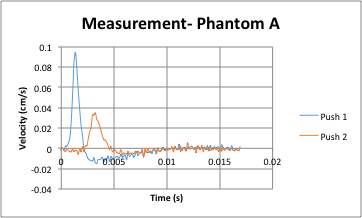
\includegraphics[width=0.5\linewidth]{steve/figs/image16.png} &
        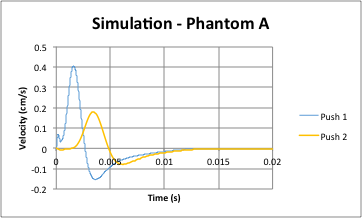
\includegraphics[width=0.5\linewidth]{steve/figs/image17.png} \\
    \end{tabular}
    \caption{LEFT: Representative shear wave measurements from the Phase II Set
        1 phantoms.  RIGHT: Matched viscoelastic shear wave simulation.}
\label{fig:steve-phantomA}
\end{figure}
